\documentclass[10pt]{article}
\usepackage[letterpaper,margin=0.43in]{geometry}
\usepackage{times}
\usepackage{graphicx}
\usepackage{booktabs}
\usepackage{array}
\usepackage{enumitem}
\usepackage{hyperref}
\usepackage{caption}
\usepackage{multicol}

\pagestyle{empty}
\linespread{0.93}
\captionsetup{font=footnotesize,labelfont=bf,skip=2pt}
\setlength{\abovecaptionskip}{1pt}
\setlength{\belowcaptionskip}{0pt}
\setlength{\parindent}{0pt}
\setlength{\parskip}{1pt}
\setlength{\columnsep}{0.18in}
\setlist[itemize]{leftmargin=*,topsep=1pt,itemsep=0pt,parsep=0pt}

\begin{document}
\footnotesize

\begin{center}
{\Large \textbf{AI-Driven Candidate Search on Top of A.S.E}}\\[-1pt]
{\normalsize Jiawen Liu, MBZUAI \quad CS7602/CS8602 Final Case Study}
\end{center}
\vspace{-0.25em}

\textbf{Problem and motivation.}
A.S.E (AICGSecEval) is a repository-level benchmark for evaluating security in AI-generated code. It already provides the core evaluation pipeline, but the course project requires an AI-search setting: define many candidate solutions, run a fixed evaluator repeatedly, and use feedback to improve future candidates. My contribution is therefore not a new security scanner; it is an experimental layer that turns A.S.E into a repeatable candidate-search benchmark.

\textbf{Research questions.}
This case study asks: (RQ1) can an AI proposer find better repository-level patch-generation settings than random or static baselines under the same run budget? (RQ2) does feedback-driven prompt refinement improve the distribution of A.S.E scores, or only produce isolated high-scoring runs? A candidate is treated as a complete experimental configuration, including retrieval, context packing, prompt style, and generation parameters.

\begin{multicols}{2}
\raggedcolumns

\textbf{What was added beyond A.S.E.}
\begin{itemize}
  \item A stable \texttt{evaluate(candidate)} wrapper around upstream \texttt{invoke.py}.
  \item Candidate JSONs that control retrieval \texttt{top\_k}, README inclusion, prompt template, temperature, and generation length.
  \item Batch runners for many candidates, repeats, resumability, and log redaction.
  \item AI-driven candidate generation in two forms: general parameter search and prompt-iterative optimization.
  \item Analysis scripts that produce per-run tables, candidate rankings, and iteration plots.
\end{itemize}

\textbf{Experimental design.}
Four schemes were compared under the same A.S.E evaluator and dataset slice:
\textbf{AI General Search}, \textbf{AI Prompt-Iterative}, \textbf{Random Baseline}, and \textbf{Static Baseline}. Each scheme has 16 completed runs. The headline metric is the official A.S.E \texttt{overall} score. Auxiliary continuous metrics were used only for exploration and are not the main reported score.
The run budget is intentionally small enough to be reproducible on a course server, but large enough to compare search behavior across multiple rounds rather than a single lucky candidate.

\textbf{Main quantitative result.}

\begin{center}
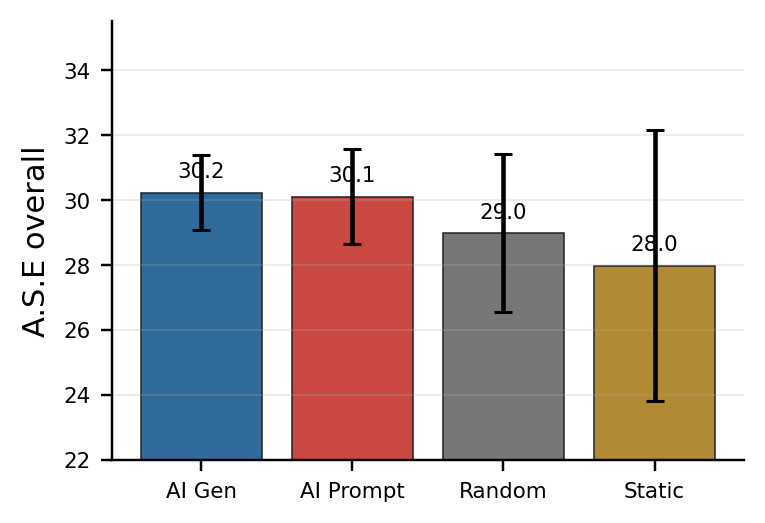
\includegraphics[width=0.82\linewidth]{figures/compare_4way_ase_compact.png}
\captionof{figure}{Official A.S.E overall score, mean $\pm$ standard deviation.}
\end{center}

\begin{center}
\scriptsize
\begin{tabular}{@{}p{0.33\linewidth}rrrr@{}}
\toprule
Scheme & Mean & Std & Best & $\Delta$ Static \\
\midrule
AI General & 30.22 & 1.14 & 34.08 & +2.25 \\
AI Prompt & 30.10 & 1.46 & 34.08 & +2.13 \\
Random & 28.97 & 2.43 & 30.10 & +1.00 \\
Static & 27.97 & 4.17 & 30.10 & 0.00 \\
\bottomrule
\end{tabular}
\captionof{table}{Official A.S.E overall score over 16 runs per scheme.}
\end{center}

\textbf{Concrete observations.}
\begin{itemize}
  \item Both AI schemes outperform random and static baselines on mean official score.
  \item AI General Search has the best mean score (30.22), but the margin over AI Prompt-Iterative is small (0.13).
  \item AI schemes reduce variance substantially: AI General std is 1.14 versus Static std 4.17, suggesting more stable candidates under this budget.
  \item Both AI schemes find a best run of 34.08, while random/static peak at 30.10. This supports the search value, even though the mean gain is modest.
\end{itemize}

\columnbreak

\textbf{Iteration-level view.}

\begin{center}
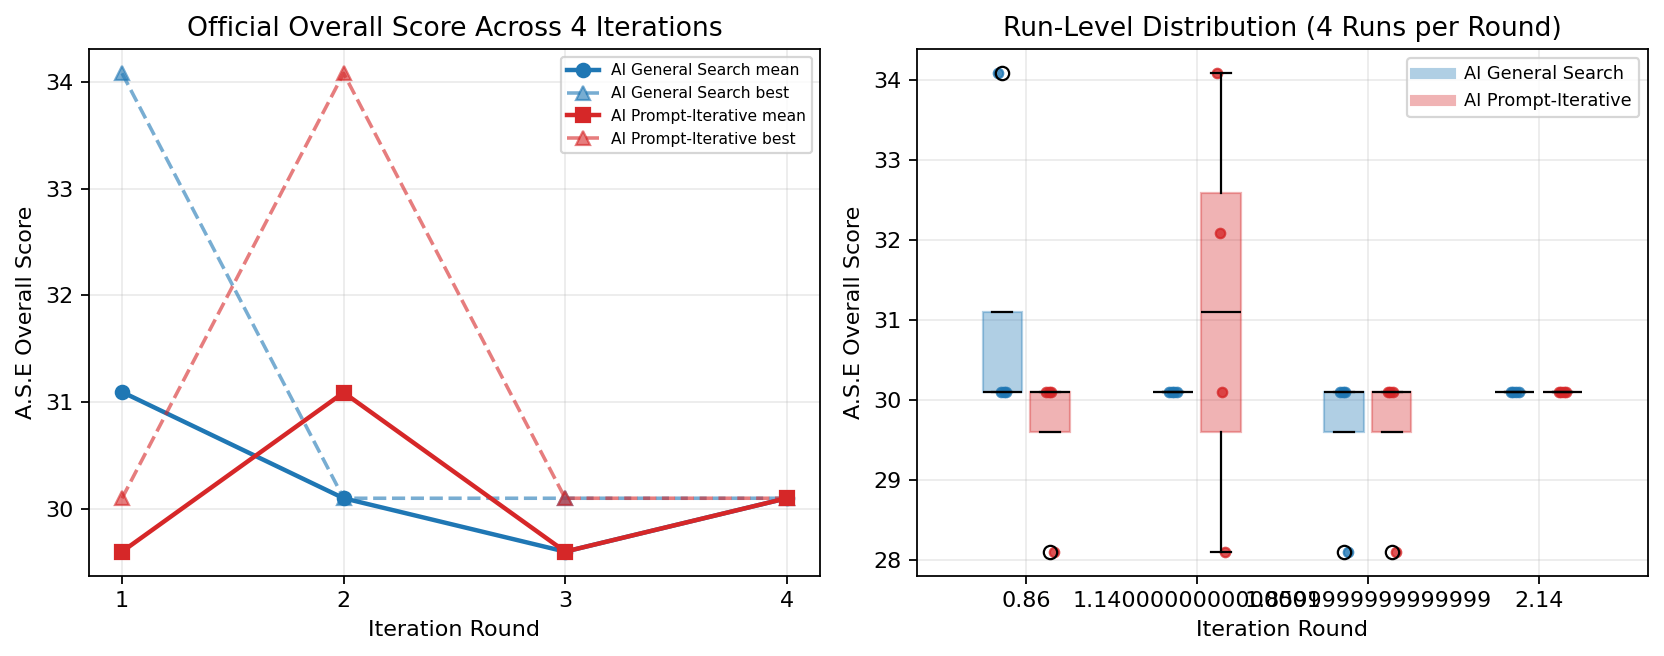
\includegraphics[width=0.98\linewidth]{figures/ai_rounds_overall.png}
\captionof{figure}{Four-round view using official A.S.E overall. The trend is not monotonic; improvements appear as discrete search hits.}
\end{center}

\begin{center}
\scriptsize
\begin{tabular}{@{}lrrrr@{}}
\toprule
Route & R1 & R2 & R3 & R4 \\
\midrule
AI General mean & 31.10 & 30.10 & 29.60 & 30.10 \\
AI General best & 34.08 & 30.10 & 30.10 & 30.10 \\
AI Prompt mean & 29.60 & 31.09 & 29.60 & 30.10 \\
AI Prompt best & 30.10 & 34.08 & 30.10 & 30.10 \\
\bottomrule
\end{tabular}
\captionof{table}{Round-by-round official A.S.E overall score.}
\end{center}

\textbf{Interpretation.}
The results show an important pattern: iteration does not produce a smooth upward curve, but it does find higher-scoring candidates than random/static baselines under the same run budget. This is expected for repository-level security evaluation because the official score is coarse and many candidate changes map to the same pass/fail outcomes. The useful signal is therefore not a clean monotonic trend; it is that AI-guided search reaches better best-case candidates and lower variance than non-AI baselines.

\textbf{Metric clarification.}
\texttt{overall\_mean}, \texttt{overall\_std}, and \texttt{best\_overall} are official A.S.E metrics. \texttt{combined}, \texttt{contrast}, and \texttt{refined} are our auxiliary metrics; they are excluded from the headline table to avoid mixing benchmark scoring with our own ranking heuristic.

\textbf{Limitations and next step.}
The current task slice is still small, and the official score is clustered. A stronger final experiment should expand tasks/CWEs while keeping the same evaluator, and then report both official A.S.E means and auxiliary diagnostics as separate analyses.

\textbf{Artifacts.}
Code and outputs are in \texttt{scripts/}, \texttt{configs/}, and \texttt{outputs\_final/analysis\_compare/}.

\end{multicols}

\vspace{0.45em}
\hrule
\vspace{0.45em}

\begin{minipage}[t]{0.49\textwidth}
\textbf{Evaluator workflow.}
Each candidate is evaluated as a complete repository-level patching attempt. The wrapper first materializes a candidate configuration, creates a batch directory, and calls the upstream A.S.E command in LLM mode. A.S.E then retrieves repository context, asks the model to generate a unified diff, applies the generated patch, and runs the benchmark's quality and security checks. The wrapper parses the resulting artifacts into a normalized \texttt{summary.json} so that every run has the same schema, including candidate id, batch id, runtime, official scores, logs, and raw artifact paths. Failed runs are still recorded rather than silently dropped, which matters for search because failures are part of the candidate quality signal.

\textbf{Why fixed evaluation matters.}
The evaluator is deliberately kept fixed after the experiment starts. Candidate search changes the solution proposal, not the scoring rule. This makes the comparison closer to a black-box optimization problem: each candidate receives a score from the same A.S.E pipeline, and the search process must learn which retrieval, prompting, and generation choices are promising under that fixed objective.
\end{minipage}
\hfill
\begin{minipage}[t]{0.49\textwidth}
\textbf{AI-driven loop.}
The AI component receives previous result tables and proposes the next candidate batch. In the general-search route, it changes parameters such as \texttt{top\_k}, README inclusion, prompt template, temperature, and max tokens. In the prompt-iterative route, the non-prompt settings are kept closer to a baseline while the prompt is revised using feedback from previous rounds. Random and static baselines provide controls: random tests whether improvement comes from simply sampling more configurations, while static tests whether a single reasonable configuration is enough.

\textbf{Main takeaway.}
The final evidence is modest but usable for a one-page case study. AI search does not show a clean monotonic learning curve, but it produces a better candidate distribution: higher official mean score than both baselines, higher best observed score, and lower variance than the static baseline. The most defensible conclusion is therefore that AI guidance is useful as a candidate generator under a limited run budget, while stronger claims require a larger task/CWE set and more repeats.
\end{minipage}
\end{document}
